% Updated ER Diagram — University Enrolment & Lecture Management System
%
% MSE800 — Professional Software Engineering
% Week 3, Activity 4: PostgreSQL project
%
% This document reviews and updates the starting ER diagram (starting-ER.png)
% and re-draws it in Chen notation using TikZ.
%
% Compile with:  pdflatex er_diagram.tex   (or lualatex / xelatex)
%
\documentclass[11pt]{article}

\usepackage[margin=0.8in]{geometry}
\usepackage{tikz}
\usetikzlibrary{shapes.geometric, backgrounds}
\usepackage{booktabs}
\usepackage[T1]{fontenc}

% ---------------------------------------------------------------- TikZ styles
\tikzset{
  entity/.style = {
    rectangle, draw=black, thick, rounded corners=2pt,
    minimum width=2.7cm, minimum height=0.9cm,
    align=center, font=\bfseries, fill=blue!10
  },
  attrib/.style = {
    ellipse, draw=black, align=center, font=\small,
    minimum height=0.7cm, inner sep=3pt, fill=yellow!12
  },
  rel/.style = {
    diamond, draw=black, thick, align=center, font=\small,
    minimum size=1.1cm, inner sep=0pt, fill=orange!15
  },
  card/.style = {
    font=\small\bfseries, fill=white, inner sep=1pt
  },
  edge/.style = { draw=black, thick }
}

\begin{document}

\title{\textbf{Updated ER Diagram}\\[4pt]
\large University Enrolment \& Lecture Management System}
\author{Nick Jones}
\date{MSE800 --- Week 3, Activity 4}
\maketitle

\section*{Relationships}

The model contains two relationships. Both are \emph{ternary} relationships in
the source diagram; each is described below together with its cardinalities.

\begin{description}
  \item[\textbf{Enrolls} --- Student : Enrollment : Lecture.]
    A \textbf{Student} \emph{enrolls in} a \textbf{Lecture} through an
    \textbf{Enrollment} record. This is a \emph{many-to-many} association
    between \emph{Student} and \emph{Lecture}, resolved by the associative
    entity \emph{Enrollment}:
    \begin{itemize}
      \item one \emph{Student} may have \emph{many} enrollments ($M$);
      \item one \emph{Lecture} may be taken by \emph{many} students ($M$);
      \item each \emph{Enrollment} links exactly \emph{one} student to exactly
            \emph{one} lecture ($1$).
    \end{itemize}

  \item[\textbf{Lectures} --- Lecturer : Lecture : Subjects.]
    A \textbf{Lecturer} \emph{delivers} a \textbf{Lecture} that belongs to a
    particular \textbf{Subject}. This ternary relationship decomposes into two
    \emph{one-to-many} associations that meet at \emph{Lecture}:
    \begin{itemize}
      \item one \emph{Lecturer} delivers \emph{many} lectures ($1:N$);
      \item one \emph{Subject} has \emph{many} lectures ($1:N$);
      \item each \emph{Lecture} is delivered by exactly \emph{one} lecturer and
            belongs to exactly \emph{one} subject ($1$).
    \end{itemize}
\end{description}

\section*{Changes from the original diagram}

\begin{itemize}
  \item \textbf{Added} an \texttt{Email} attribute to \emph{Student},
        \texttt{Credits} and \texttt{Description} attributes to \emph{Subjects}, a
        \texttt{Room} attribute to \emph{Lecture}, and a \texttt{Grade} attribute
        to \emph{Enrollment}.
  \item \textbf{Corrected} the \emph{Lecturer} key: \texttt{Lecture\_id} becomes
        \texttt{Lecturer\_id} (a lecturer is identified by their own id, not by a
        lecture).
  \item \textbf{Corrected} the \emph{Enrollment} key: \texttt{Student\_code} alone
        cannot identify an enrollment (a student may enrol in several courses), so
        a surrogate \texttt{Enrollment\_id} primary key is introduced.
  \item \textbf{Resolved} the overlapping course attributes
        (\texttt{CC\#} / \texttt{Subject} / \texttt{Subject\_code}) into a single
        foreign key to the \emph{Subjects} entity.
\end{itemize}

\section*{ER Diagram}

\begin{figure}[h]
  \centering
  \resizebox{\textwidth}{!}{%
  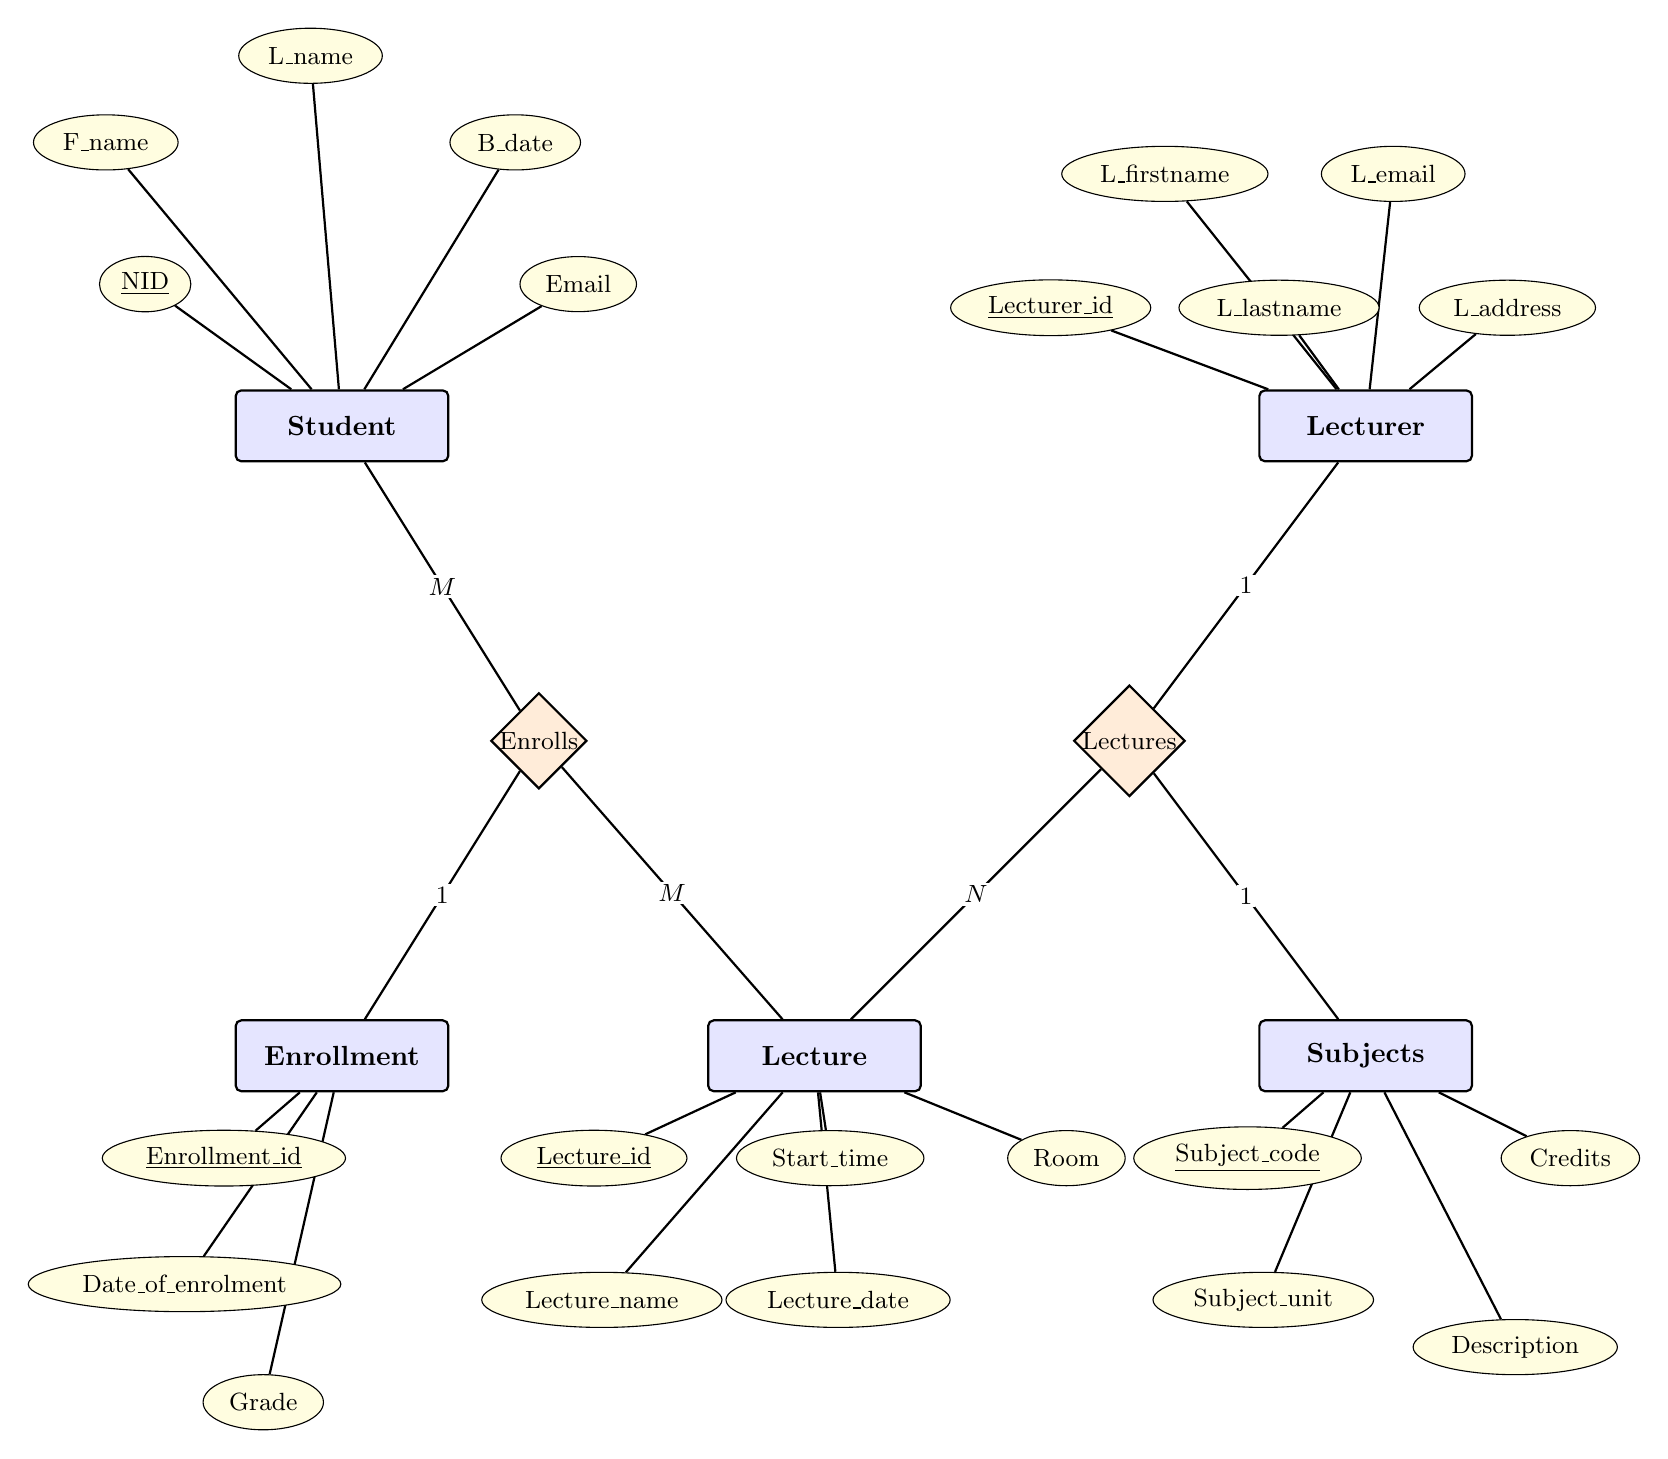
\begin{tikzpicture}[node distance=0.4cm]

    % ------------------------------------------------------------- Entities
    \node [entity] (student)    at (2,  11) {Student};
    \node [entity] (enrollment) at (2,   3) {Enrollment};
    \node [entity] (lecture)    at (8,   3) {Lecture};
    \node [entity] (lecturer)   at (15, 11) {Lecturer};
    \node [entity] (subjects)   at (15,  3) {Subjects};

    % -------------------------------------------------------- Relationships
    \node [rel] (enrolls)  at (4.5, 7) {Enrolls};
    \node [rel] (lectures) at (12,  7) {Lectures};

    % ------------------------------------------------- Student attributes
    \node [attrib] (nid)      at (-0.5, 12.8) {\underline{NID}};
    \node [attrib] (f_name)   at (-1.0, 14.6) {F\_name};
    \node [attrib] (l_name)   at ( 1.6, 15.7) {L\_name};
    \node [attrib] (b_date)   at ( 4.2, 14.6) {B\_date};
    \node [attrib] (email)    at ( 5.0, 12.8) {Email};

    % ------------------------------------------------ Enrollment attributes
    \node [attrib] (enr_id)   at (0.5, 1.7) {\underline{Enrollment\_id}};
    \node [attrib] (enr_date) at (0.0, 0.1) {Date\_of\_enrolment};
    \node [attrib] (grade)    at (1.0, -1.4) {Grade};

    % -------------------------------------------------- Lecture attributes
    \node [attrib] (lec_id)   at (5.2,  1.7) {\underline{Lecture\_id}};
    \node [attrib] (lec_name) at (5.3, -0.1) {Lecture\_name};
    \node [attrib] (stime)    at (8.2,  1.7) {Start\_time};
    \node [attrib] (ldate)    at (8.3, -0.1) {Lecture\_date};
    \node [attrib] (room)     at (11.2, 1.7) {Room};

    % ------------------------------------------------- Lecturer attributes
    \node [attrib] (ltr_id)   at (11.0,  12.5) {\underline{Lecturer\_id}};
    \node [attrib] (l_fname)  at (12.45, 14.2) {L\_firstname};
    \node [attrib] (l_lname)  at (13.9,  12.5) {L\_lastname};
    \node [attrib] (l_email)  at (15.35, 14.2) {L\_email};
    \node [attrib] (l_addr)   at (16.8,  12.5) {L\_address};

    % -------------------------------------------------- Subjects attributes
    \node [attrib] (subj_code) at (13.5,  1.7) {\underline{Subject\_code}};
    \node [attrib] (subj_unit) at (13.7, -0.1) {Subject\_unit};
    \node [attrib] (subj_udsc) at (16.9, -0.7) {Description};
    \node [attrib] (credits)   at (17.6,  1.7) {Credits};

    % ----------------------------------------- Connectors (behind the shapes)
    \begin{scope}[on background layer]

      % -------- relationship connectors
      \draw [edge] (student)   -- (enrolls)  node [card, pos=0.5] {$M$};
      \draw [edge] (enrollment)-- (enrolls)  node [card, pos=0.5] {$1$};
      \draw [edge] (lecture)   -- (enrolls)  node [card, pos=0.5] {$M$};
      \draw [edge] (lecturer)  -- (lectures) node [card, pos=0.5] {$1$};
      \draw [edge] (lecture)   -- (lectures) node [card, pos=0.5] {$N$};
      \draw [edge] (subjects)  -- (lectures) node [card, pos=0.5] {$1$};

      % -------- student
      \draw [edge] (student) -- (nid);
      \draw [edge] (student) -- (f_name);
      \draw [edge] (student) -- (l_name);
      \draw [edge] (student) -- (b_date);
      \draw [edge] (student) -- (email);

      % -------- enrollment
      \draw [edge] (enrollment) -- (enr_id);
      \draw [edge] (enrollment) -- (enr_date);
      \draw [edge] (enrollment) -- (grade);

      % -------- lecture
      \draw [edge] (lecture) -- (lec_id);
      \draw [edge] (lecture) -- (lec_name);
      \draw [edge] (lecture) -- (stime);
      \draw [edge] (lecture) -- (ldate);
      \draw [edge] (lecture) -- (room);

      % -------- lecturer
      \draw [edge] (lecturer) -- (ltr_id);
      \draw [edge] (lecturer) -- (l_fname);
      \draw [edge] (lecturer) -- (l_lname);
      \draw [edge] (lecturer) -- (l_email);
      \draw [edge] (lecturer) -- (l_addr);

      % -------- subjects
      \draw [edge] (subjects) -- (subj_code);
      \draw [edge] (subjects) -- (subj_unit);
      \draw [edge] (subjects) -- (subj_udsc);
      \draw [edge] (subjects) -- (credits);

    \end{scope}

  \end{tikzpicture}
  }
  \caption{Updated ER diagram in Chen notation. Primary keys are underlined.
           Foreign keys are carried by the relationships rather than shown as
           attributes.}
\end{figure}

\noindent\textbf{Legend:} rectangles are entities, diamonds are relationships,
ellipses are attributes, and underlined attributes are primary keys.

\end{document}
